\chapter{Introduction}
\label{chap:intro}

\section{Background and Motivation}

\emph{Wireless sensor network} (WSN)~\cite{wsn_survey} is a network of spatially dispersed and dedicated sensors that monitor and record the 
physical conditions of the environment and forward the collected data to a central location via wireless communication.
WSN can measure environment conditions such as temperature, sound, humidity, wind, light, wireless channel state information and radio spectrum, etc.
A sensor network becomes a \emph{quantum sensor network} (QSN) when the sensors leverage quantum objects and quantum properties~\cite{RevModPhys.quantumsensing}
such as quantum coherance, quantum entanglement.
Quantum sensors are extremely sensitive to physical quantities such as magnetic field, electric field, quadrature displacement
and phase shift in the optic field.

\para{Classical sensors}. WSNs have various applications~\cite{tsn17-water,sensys10-health,mobicom03-sensor}.
In this thesis, the application we focus on is spectrum surveillance and monitoring~\cite{arani2018} for security and threat detection.
The \emph{core problem} involved in this application is \emph{transmitter localization}~\cite{ton-sensorselect,caitao2023qsn}, and in particular, multiple transmitter localization (\mtl) as 
the number of transmitter present in an area could be more than one and localizing multiple transmitters are not independent.
The reason for being not independent is that a sensor receives an aggregated power from multiple transmitters and separating 
the power from different multiple sources is impractical.
That an aggregated received power not able to separete is a big challenge for \mtl.
Furthermore, in a shared spectrum paradigm, presence of an evolving set of authorized users 
(e.g., primary and secondary users) adds to the challenge.

The shared spectrum paradigm composes an important background for our \mtl work.
The RF spectrum is a natural resource in great demand due to the unabated increase in mobile (and hence, wireless) data consumption~\cite{Jeffrey14}. 
The research community has addressed this capacity crunch via development of shared spectrum paradigms, wherein the spectrum 
is made available to unlicensed users (secondaries) as long as they do not interfere with the transmission of licensed incumbents (primaries).
The fundamental objective behind such shared spectrum paradigms is to maximize spectrum utilization,
the viability of such systems depends on the ability to effectively guard the shared spectrum against unauthorized usage. 
The current mechanisms however to locate such unauthorized users (intruders) are human-intensive and time-consuming, 
involving FCC enforcement bureau which detects violations via complaints and manual investigation~\cite{mobicom17-splot}. 

\begin{figure}[t]
      \centering
      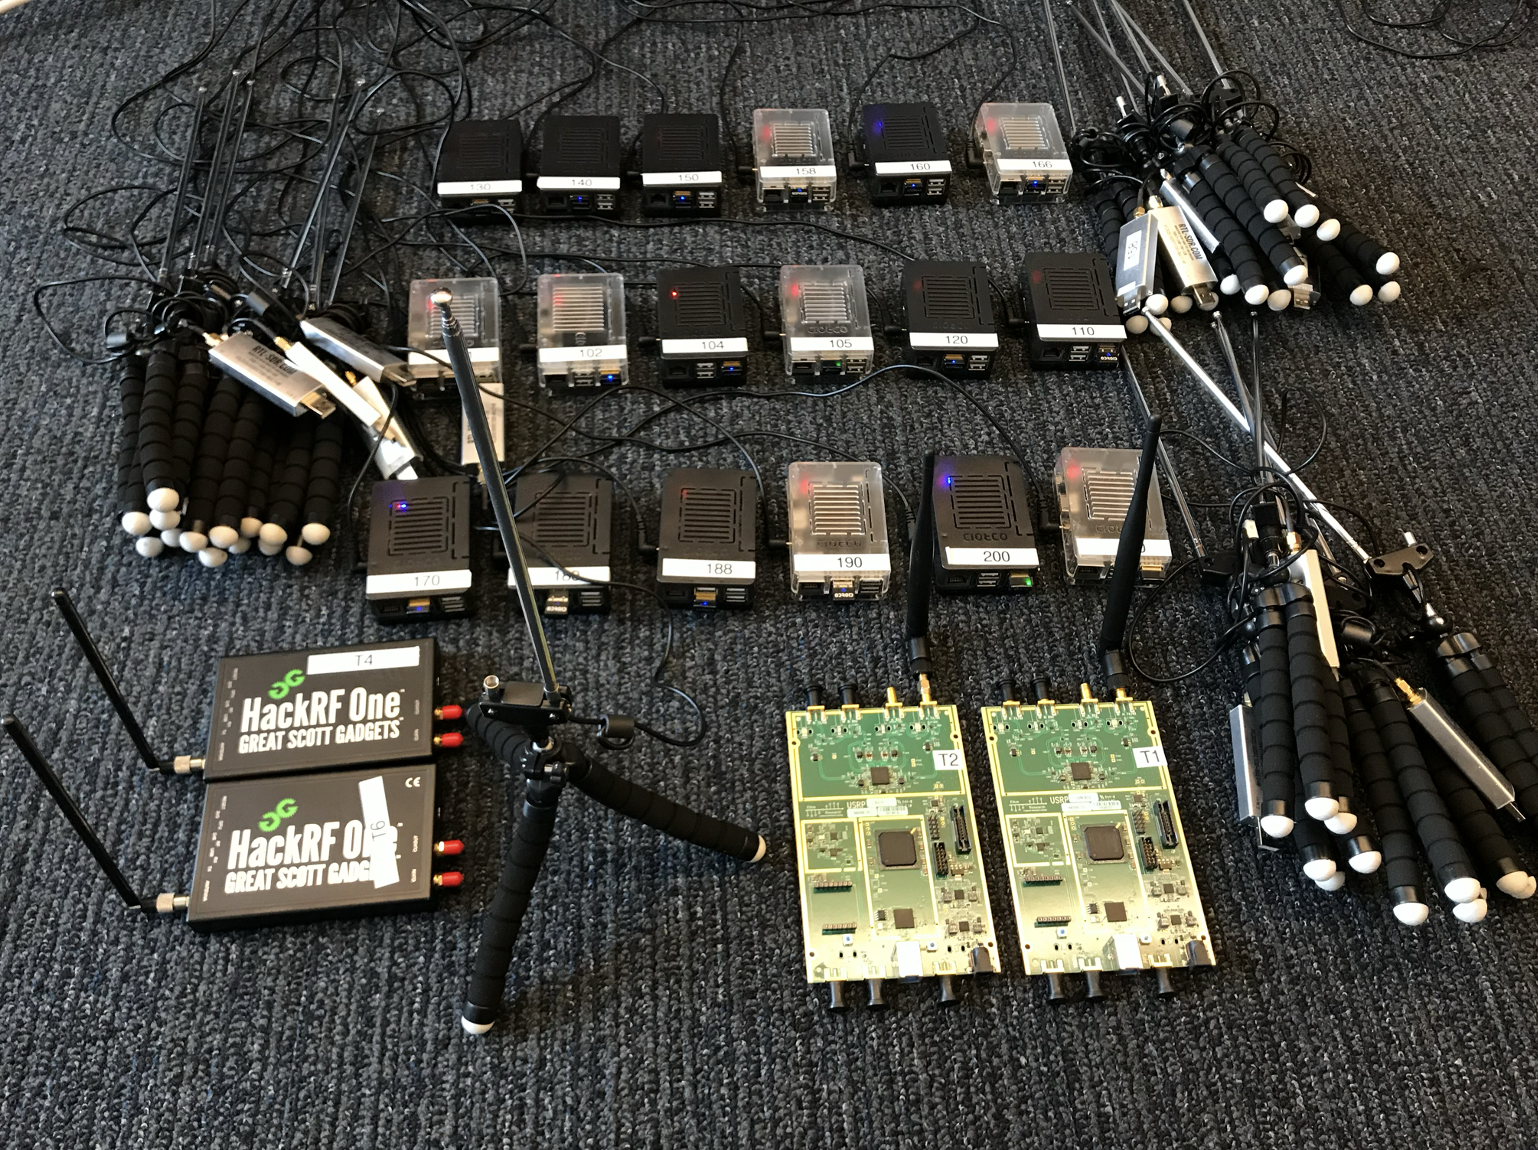
\includegraphics[width=0.7\textwidth]{figures/SDR.png}
      \caption{Classical sensors. Radio frequency sensors used in this thesis. Details see~\S\ref{sec:testbed}} 
      \label{fig:intro-sdr}
\end{figure}

Motivated by above, we seek for an effective technique that is able to accurately localize multiple simultaneous
intruders and even in the presence of dynamically changing set of authorized users.
Our solution assumes a network of crowdsourced sensors wherein relatively low-cost spectrum sensors are available
for gathering signal strength in the form of received power.
We introduce two different approaches to the \mtl problem.
The first approach is a hypothesis-driven Bayesian approach, viz. maximum a posterior approach, where wherein each hypothesis is a configuration
(i.e. a combination of $\langle$location, power$\rangle$ pair of the potential intruders), and the goal is to determine the hypothesis 
that best explains the sensor observations.
The second approach is a deep learning-based approach. First, we encode the sensors' observation data into an image.
Then, we frame \mtl as a sequence of two steps: image-to-image translation 
and object detection, each of which is solved using a trained CNN model. 
The first step of image-to-image translation maps an input image representing sensor readings to an image
representing the distribution of transmitter locations, and the second object detection step derives precise locations of
transmitters from the image of transmitter distributions. 
Besides the location, the transmission power is another property of a transmitter that we wish to estimate.
We introduces some novel methods to estimate the power of multiple transmitters.
We also introduce a novel interapolation method for received signal strength.



\para{Quantum sensors.}
In the quantum side, we use QSN, instead of WSN, to continue solving the problem of transmitter localization.
Albeit classical sensors are omnipresent, there are big motivations to explore quantum sensors.
Quantum sensing is an emerging field that leverages the quantum properties of light and matter at atomic/subatomic scales and has the potential to sense signals at an unprecedented level of precision.
Quantum sensing brings new opportunities to new and well-established problems.
For example, physicists in the year 2016 used squeezed quantum states to improve the sensitivity of the Laser Interferometer Gravitational-wave Observatory (LIGO) detector and successfully detected gravitational waves.
In~\cite{PRL20-qsn}, researchers use some distributed quantum RF-photonic sensors to estimate the amplitude and phase of a radio signal.
They showed the performance of sensing a global property of the RF wave is enhanced by leveraging a shared multipartite entangled state produced by squeezed light.
In their experiments, the estimation variance of RF amplitude and phase both beat the standard quantum limit by over 3 dB.
The precision improvement factor of $1/\sqrt{N}$ for $N$ sensors is known as reaching the Heisenberg limit.

\begin{figure}[t]
      \centering
      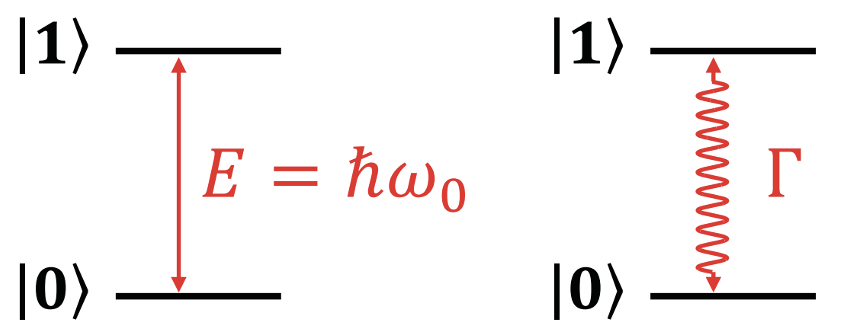
\includegraphics[width=0.5\textwidth]{figures/qsensor.png}
      \caption{Quantum sensor theory. Basic features of a two-state quantum sensor, figure from~\cite{RevModPhys.quantumsensing}.
               $\ket{0}$ is the lower energy state and $\ket{1}$ is the higher energy state. Quantum sensing leverages changes in the
               transition frequence $\omega_{0}$ (shifts of the energy level) or the transition rate (transition between energy levels) 
               in reponse to an external signal $V$.} 
      \label{fig:intro-qsensor}
\end{figure}

\begin{figure}[t]
      \centering
      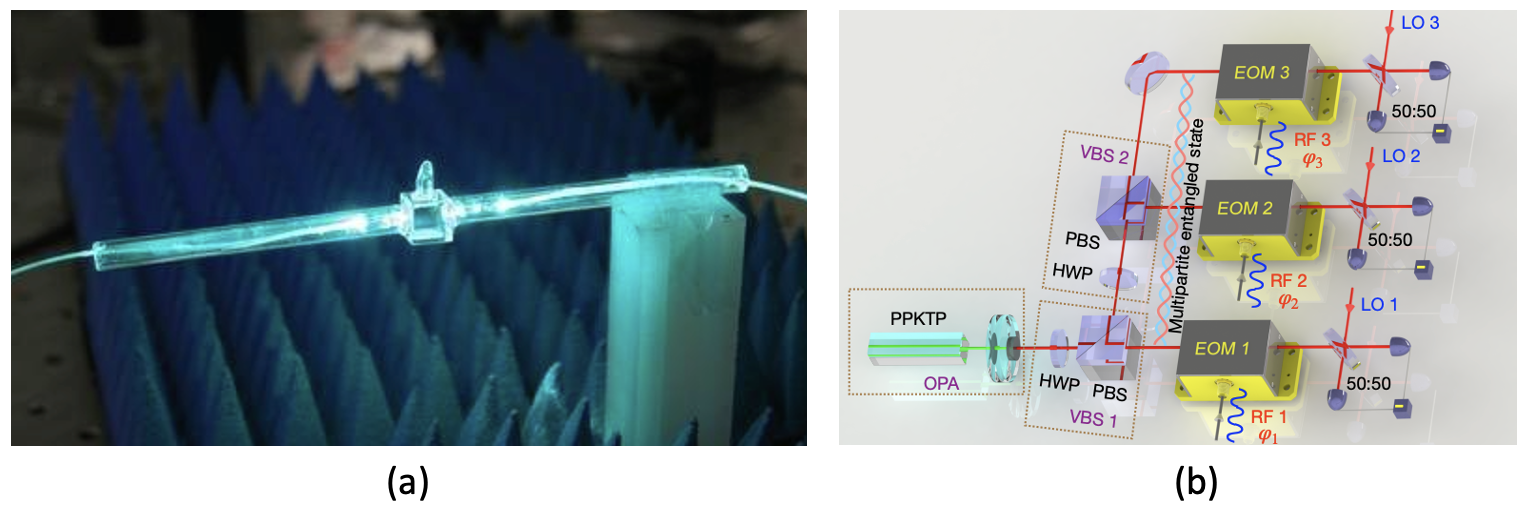
\includegraphics[width=0.85\textwidth]{figures/qsensor2.png}
      \caption{Quantum sensors. (a) Fiber-coupled vapor cell for Electric field measurements using Rydberg atoms;
               (b) Reconfigurable entangled radio frequency photonic sensor network, figure from~\cite{PRL20-qsn}.} 
      \label{fig:intro-qsensor2}
\end{figure}

Motivated by the above, we aim to leverage quantum sensors to perform some canonical tasks and thus open a new avenue of research.
The canonical task we picked is RF transmitter localization~\cite{nsdi13-arraytrack,pmc22-deepmtlpro}.
We consider a network of quantum sensors distributed in a geographic area and a single transmitter active in the area to be localized.
We pose the localization problem as a quantum state discrimination problem~\cite{bergou-review-2007}. 
In our approach, the quantum sensor network reports a quantum state, and we discriminate the quantum state via 
positive-operator valued measure (POVM) and the POVM's output indicates the transmitter location.
The key challenge here is the scalability challenge, i.e., the method's time and space complexity grows exponentially against the
number of sensors and the method's localization accuracy decrease against the number of discrete locations.
To solve the challenge, we propose a two-level POVM method that is comprised of a coarse-level POVM and a fine-level POVM.
The two level idea is effective and can be generalized into three levels and more.

Quantum entanglement is a phenomenon that has no counterpart in the classical world.
It is the physical phenomenon that occurs when a group of particles (electrons, photons, etc) are generated, interact, or share spatial proximity in a way such that
the quantum state of each particle of the group cannot be described independently of the state of the others, including when the particles
are separated by a large distance.
In short, quantum entanglement is a specially strong correlation between multiple particles.
In our context of QSNs, entanglement can be served as a resource to enhance the perforance of the QSN.
For example, the $1 / \sqrt{N}$ improvement factor mentioned above requires the initial probe state as an entangled state.
The entanglement pair resource is generated at a single node, but the quantum sensors are spatially distributed.
Thus, a major problem is to distribute (or route) the entanglement to the quantum sensors at a potentially large distance apart.
This a challenging problem in the field of quantum communication.
Physical transmission of quantum states accross nodes can incur irreparable communication errors, as the no-cloning theorem proscribes
making independent copies of arbitrary qubits.
The establish of entanglement over long distance is challenging due to the low probability of success of the underlying physical process
(short distance entanglement and swapping).
In this thesis, we propose an efficient heuristic approach that efficiently route an entanglement pair in a quantum network.

Finally, we investigate a problem that is unique in quantum, i.e., optimizing the initial state of detector sensors 
in quantum sensor networks. We consider a network of quantum sensors, where each sensor is a qubit detector that “fires”, 
i.e., its state changes when an event occurs close by. The change in state due to the firing of a detector is given 
by a unitary operator. The determination of the firing sensor can be posed as a QSD problem which incurs a probability 
of error depending on the initial state and the measurement operator used. We address the problem of determining 
the optimal initial state of the quantum sensor network that incur a minimum probability of error in determining the firing sensor.


\section{Thesis Statement}

\emph{Transmitters can be localized efficiently and accurately with our methods in classical and quantum sensor networks.}
Consider some transmitters to be localized a geographpical area. We deploy a distributed set of classical or quantum sensors in the area.
We aim to efficently and accurately localize the transmitters by processing the data received from the sensors intelligently.
Besides the core goal of transmitter localization, we also solve closely related problems such as transmission power estimation, 
receive signal strength interpolation and quantum network routing of entanglement.
\emph{Initial state can be optimized using our methods in quantum sensor networks.} 
The first step of a quantum sensing protocol is state preparation, and we propose a theory that states the optimal initial state 
for our specific problem of detector sensors in quantum sensor networks.

\section{Thesis Organization}

Towards the goal of our thesis we make the following contributions:

\begin{itemize}
    \item In Chapter~\ref{chap:ipsn}, we introduce an efficient hypothesis-based Bayesian approach \ouralgo for multiple transmitter localization (\mtl) problem (\S\ref{sec:time}); 
          A closed-form equation for the estimation of transmission power (\S\ref{sec:ipsn-power});
          A novel received signal strength interpolation method inspired from the power law distribution (\S\ref{sec:inter});
          Extend \ouralgo to accommodate the presence of authorized users (\S\ref{sec:auth}).
    
    \item In Capter~\ref{chap:wowmom-pmc}, we introduce a deep learning-based approach \our for the \mtl problem (\S\ref{sec:translate}, \S\ref{sec:detect});
          Extend \our via deep learning models to accommodate the presense of authorized users (\S\ref{sec:authorized});
          A deep learning-based approach that estimates the transmission power of multiple transmitters (\S\ref{sec:power}).
    
    \item In Chapter~\ref{chap:qce}, we introduce the concept of quantum sensor networks and the model of a quantum sensor (\S\ref{sec:quantum_problem});
          In the context of quantum sensor networks, we pose a transmitter localization problem as a quanum state discrimination problem 
          and introduce a novel quantum localization method \povm and \povmpro based on positive-operator valued measure (\S\ref{sec:povm}).
    
    \item In Chapter~\ref{chap:tqc}, we consider a network of quantum sensors, where each sensor is a qubit detector that "fires", its state changes when an event occurs close by.
          We address the problem of determining the optimal initial global state of a network of quantum sensors that incur a minimum probability of error in determining the firing sensor (\S\ref{sec:tqc_problem}).
          We have proposed both theoretical analytical results (\S\ref{sec:n-ortho}, \S\ref{sec:optimal}) and numerical simulation results(\S\ref{sec:searching}).
          
    \item In Chapter~\ref{chap:swappingtrees}, we introduce an efficient heuristic algorithm \dpalt for routing an entanglement pair.
          The algorithm is Dijkstra-based, and the path selection metric is a closed-form expression that models a path as a tree near accurately (\S\ref{sec:swapping_efficient}).
\end{itemize}


